% !TEX root = main.tex
\documentclass[a4paper, UKenglish, 11pt]{uiomaster}
\usepackage{lipsum}
\usepackage[subpreambles=true]{standalone}
\usepackage[table,xcdraw]{xcolor}

\begin{document}

\chapter{Localizing Single Dipole Sources}

As mentioned in chapter 1, an important topic in EEG signal analysis is the inverse problem of going from measured EEG signals to localized equivalent current dipoles, so-called source localization. In this chapter we will present the training and performance of the neural networks presented in chapter 4. Section ... and ... deal with training of the simple feed forward neural network and presenting its results, while section ... will discuss how a convolution neural network can be used to obtain the same results. But first, we will take a look at the dataset being fed to the different networks.

\section{Localizing Single Dipole Sources}

% One example on coordinate prediction

% include the neural net that has been used

The first problem we want to introduce for our neural network, DiLoc, is simply the standard inverse problem. By feeding the network EEG data corresponding to the electrical activity from dipoles distributed randomly in the cerebral cortex for different samples, we want the network to output the x-, y- and z-coordinates of the localization of the current dipoles. In figure \ref{fig:single_dipole_accuracy} we have provided the loss of our network as a function of training epochs. It is apparent that the the network picks up on the patterns of the data, as we clearly can observe the trend of decreasing loss with an increasing number of epochs. Moreover, we can see that the both training and validation loss stabilizes at around 400 epochs.

\begin{figure}[!htb]
    \centering
    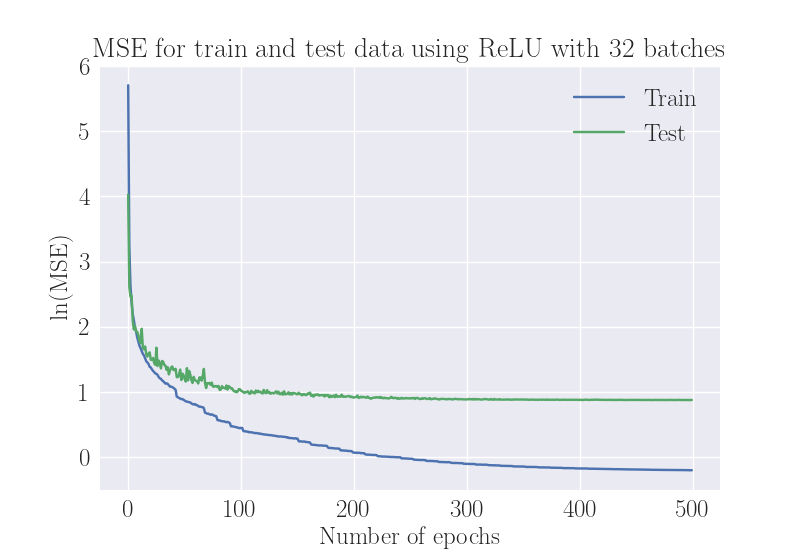
\includegraphics[width=\linewidth]{figures/MSE_simple_dipole_lr0.001_RELU_500_50000_ReLU_32_500_N_dipoles_1.png}
    \caption{The loss for the simple Feed Forward Neural Network with 50 000 samples and ReLU as activation function.}
    \label{fig:single_dipole_accuracy}
\end{figure}

In Table \ref{table:error_simple_dipole} we have provided the performance of the network by concidering different error metrics. The mean absolute error (MAE) values for the x-, y-, and z- coordinates rnage from 0.8300 mm to 0.8998 mm. This means that, on average, the network's predictions have an error smaller than 1 mm in each coordinate. Considering the range of the coordinates, the MAE values represent a reasonable level of accuracy. The mean squared error penalizes larger errors/outliers more severely than MAE since it involves squaring the differences. In our case the MSE values for the different coordinates range from 1.2134 mm to 1.4110 mm. The larger MSE values suggest that the predictions of the network may have larger errors in some cases, resulting in a higher average squared difference. However, the magnitude of the mean squared errors is still whithin a reasonable range when analyzing them in the context of the coordinates ranges. Finally the root mean squared error provides a measure of the standard deviation of the errors and helps to understand the spread of errors around the mean. The RMSE values of ours are slighly lower than the corresponding MSE values with a range from 1.1016 mm to 1.1878 mm. The table also presents the error metrics calculated for the euclidean distance. For both MAE, MSE and RMSE the value is higher than the individual coordinate errors, indicating that the errors in the x, y, and z coordinates are not perfectly aligned and contribute to the overall distance. It is worth mentioning that specific points in the cortex matrix may potentially contribute more to the errors. Further investigation could be performed to identify any specific patterns or regions in the cortex that exhibit higher error rates. However, overall the results indicate that the network is able to predict the dipole location with reasonable accuracy. While there are some errors in the predictions, the errors are generally within an acceptable range.

% Please add the following required packages to your document preamble:
% \usepackage[table,xcdraw]{xcolor}
% If you use beamer only pass "xcolor=table" option, i.e. \documentclass[xcolor=table]{beamer}
\begin{table}[!htb]
\begin{tabular}{l|cccc|}
\cline{2-5}
\rowcolor[HTML]{CBCEFB}
\cellcolor[HTML]{FFFFFF}                           & \multicolumn{4}{c|}{\cellcolor[HTML]{CBCEFB}{\color[HTML]{000000} \textbf{Error for different target values}}}                                                                                                                                                                                                                                                                                                                                                     \\ \cline{2-5}
\rowcolor[HTML]{EFEFEF}
\cellcolor[HTML]{FFFFFF}\textbf{}                  & \multicolumn{1}{l|}{\cellcolor[HTML]{EFEFEF}\begin{tabular}[c]{@{}l@{}}x-coordinate\\ {[}mm{]}\end{tabular}} & \multicolumn{1}{l|}{\cellcolor[HTML]{EFEFEF}\begin{tabular}[c]{@{}l@{}}y-coordinate \\ {[}mm{]}\end{tabular}} & \multicolumn{1}{l|}{\cellcolor[HTML]{EFEFEF}\begin{tabular}[c]{@{}l@{}}z-coordinate \\ {[}mm{]}\end{tabular}} & \multicolumn{1}{l|}{\cellcolor[HTML]{EFEFEF}\begin{tabular}[c]{@{}l@{}}Euclidean \\ Distance {[}mm{]}\end{tabular}} \\ \hline
\multicolumn{1}{|l|}{\cellcolor[HTML]{EFEFEF}MAE}  & \multicolumn{1}{c|}{0.8300}                                                                                  & \multicolumn{1}{c|}{0.8998}                                                                                   & \multicolumn{1}{c|}{0.8419}                                                                                   & 0.8573                                                                                                              \\ \hline
\multicolumn{1}{|l|}{\cellcolor[HTML]{EFEFEF}MSE}  & \multicolumn{1}{c|}{1.2638}                                                                                  & \multicolumn{1}{c|}{1.4110}                                                                                   & \multicolumn{1}{c|}{1.2134}                                                                                   & 1.2961                                                                                                              \\ \hline
\multicolumn{1}{|l|}{\cellcolor[HTML]{EFEFEF}RMSE} & \multicolumn{1}{c|}{1.1242}                                                                                  & \multicolumn{1}{c|}{1.1878}                                                                                   & \multicolumn{1}{c|}{1.1016}                                                                                   & 1.1385                                                                                                              \\ \hline
\end{tabular}
\caption{\textbf{Evaluation of the network performance utializing different Error Metrics.} \newline
Network performance on test dataset consisting of 1000 samples. The errors are measured using Mean Squared Error (MSE), Mean Absolute Error (MAE), and Root Mean Squared Error (RMSE).}
\label{table:error_simple_dipole}
\end{table}

% You can include a little bit more here. Find some examples in the figure coordinate system. Give average error in the crossection.
In order to conduct a detailed analysis of the network's performance, Figure \ref{fig:MAE_crossections} presents the Mean Absolute Error (MAE) for various dipole locations within the New York head model cortex matrix. The figure provides valuable insights into the distribution of errors across different regions of the cortex, with three cross-sections—front, top, and side—depicted for examination.

The MAE values presented in the panels are consistently below 1 mm, which indicates a high level of accuracy in the network's predictions. These results are promising and demonstrate the network's ability to estimate dipole locations with a high level of precision. The panels also offer an opportunity to assess whether the network performs differently for dipoles located in the gyrus compared to the sulcus.

Initially, it might be assumed that EEG signals originating from dipoles in the sulcus present greater challenges for the network's analysis and prediction. This assumption is based on the deeper placement of dipoles within the sulcus compared to those in the gyrus, as well as the potential complexities introduced by the dipole's orientation within the cortex. However, upon closer examination of Figure \ref{fig:MAE_crossections}, it becomes evident that the distribution of MAE values does not exhibit a clear correlation with the brain's structural characteristics. The MAE values appear to vary randomly across different regions, indicating that the network's performance is not significantly influenced by the distinction between the gyrus and sulcus.


Surprisingly, the Mean Absolute Error (MAE) for dipoles located in the sulcus is 1.1075 mm, which is even smaller than the MAE for dipoles in the gyrus measuring 1.2458 mm. This finding directly contradicts the initial assumption and suggests that the network exhibits great precision in predicting dipole locations regardless of their placement within the cortex. The lower MAE values specifically for dipoles in the sulcus  the network's remarkable ability to effectively capture the complex features and variations associated with deeper cortical placements. Moreover, the results highlight the network's robustness and accuracy across different cortical structures, reinforcing its potential for accurate dipole localization within the human brain.


\begin{figure}[!htb]
    \centering
    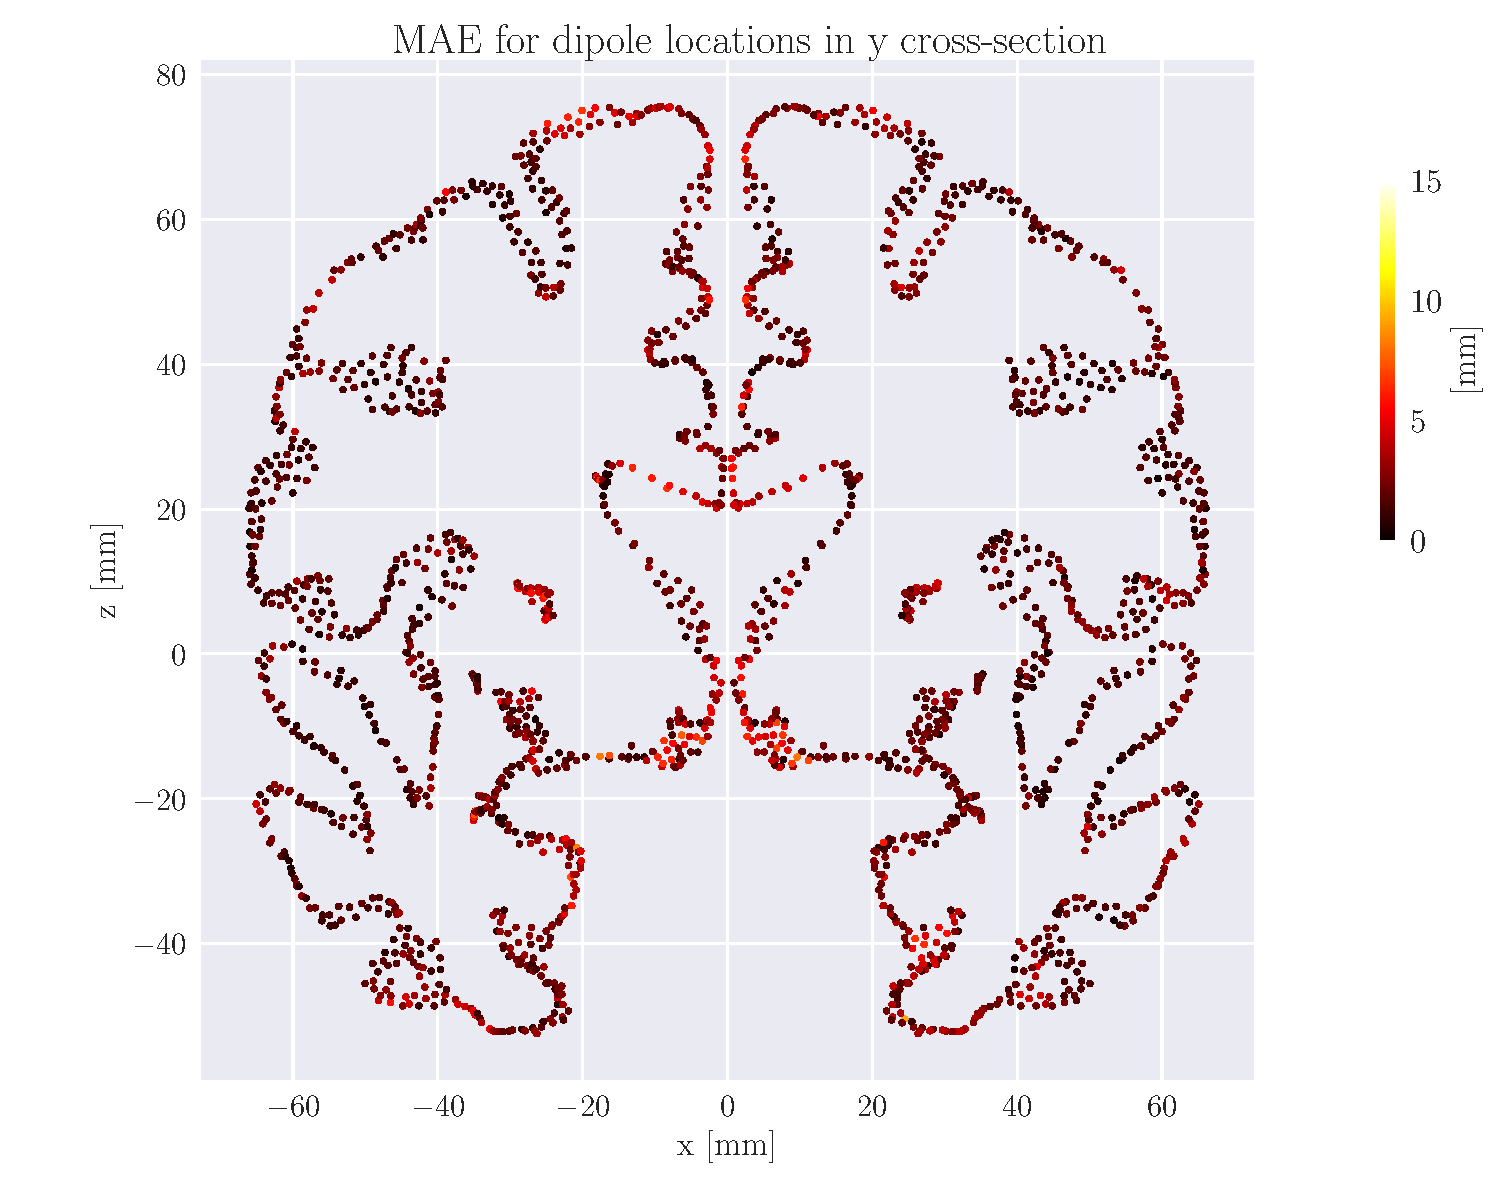
\includegraphics[width=0.7\linewidth]{figures/NEW_simple_dipole_error_Euclidean Distance_0.pdf}
    \vspace{10pt} % Adjust the vertical spacing between the images
    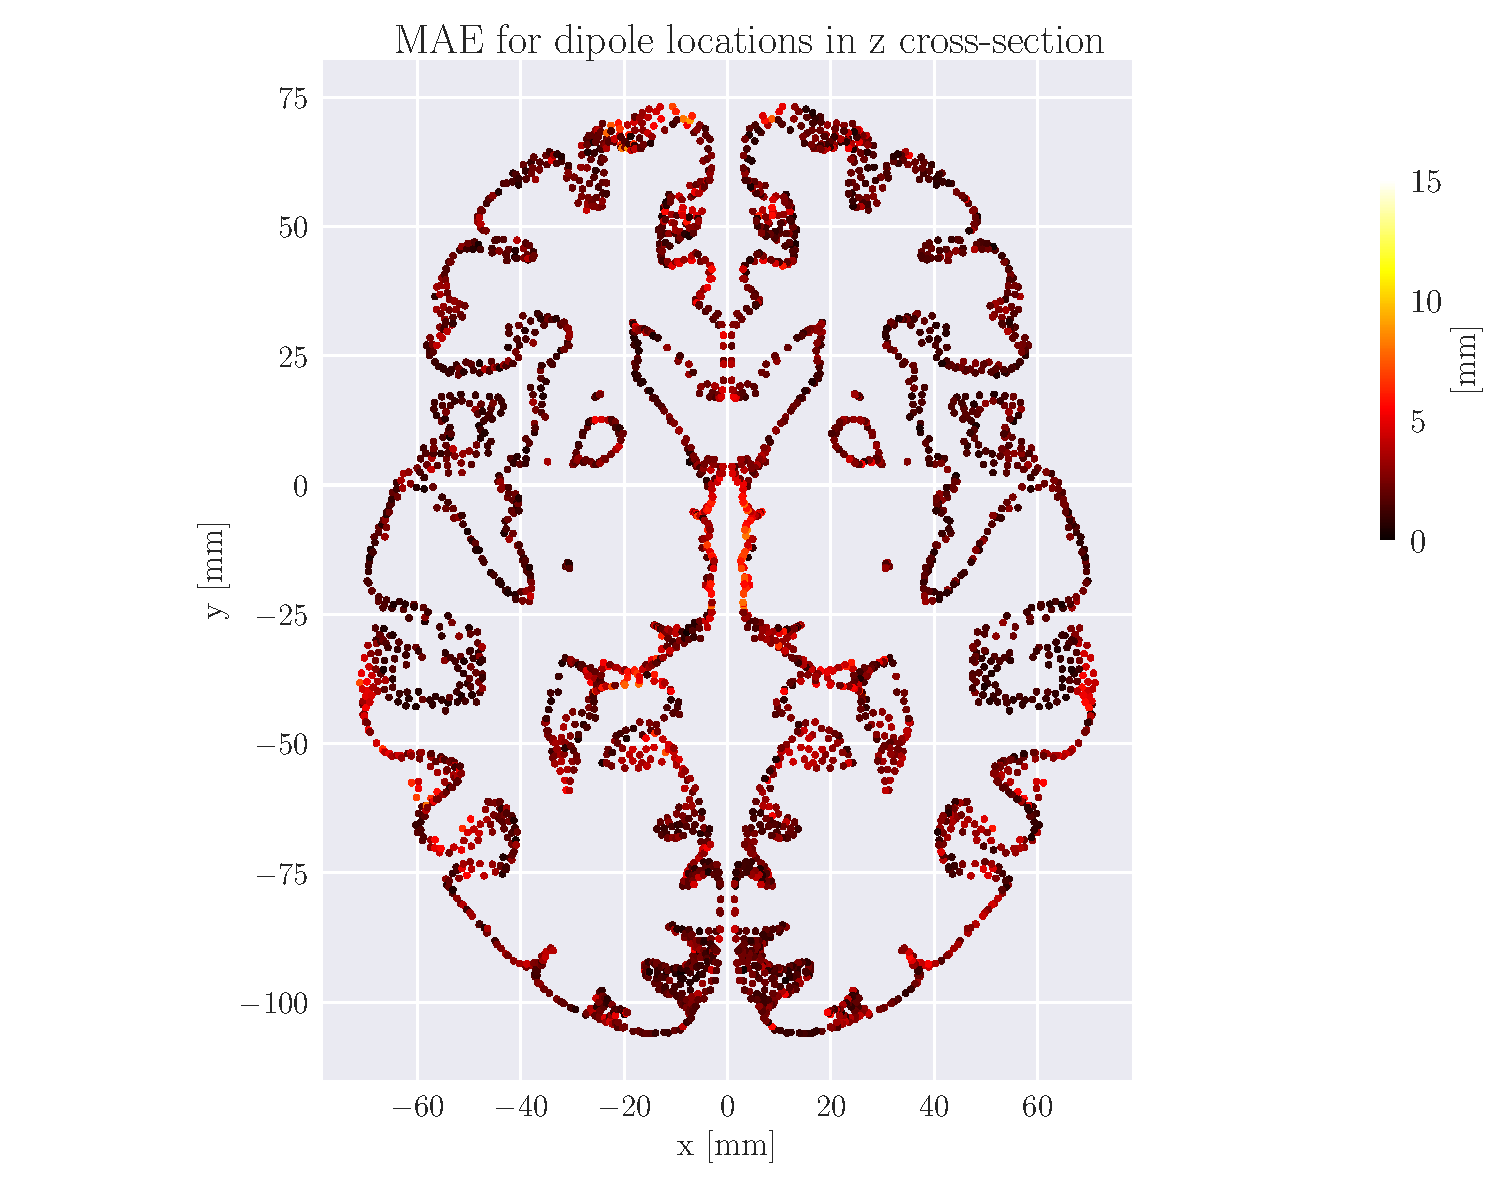
\includegraphics[width=0.7\linewidth]{figures/NEW_simple_dipole_error_Euclidean Distance_1.pdf}
    \vspace{10pt} % Adjust the vertical spacing between the images
    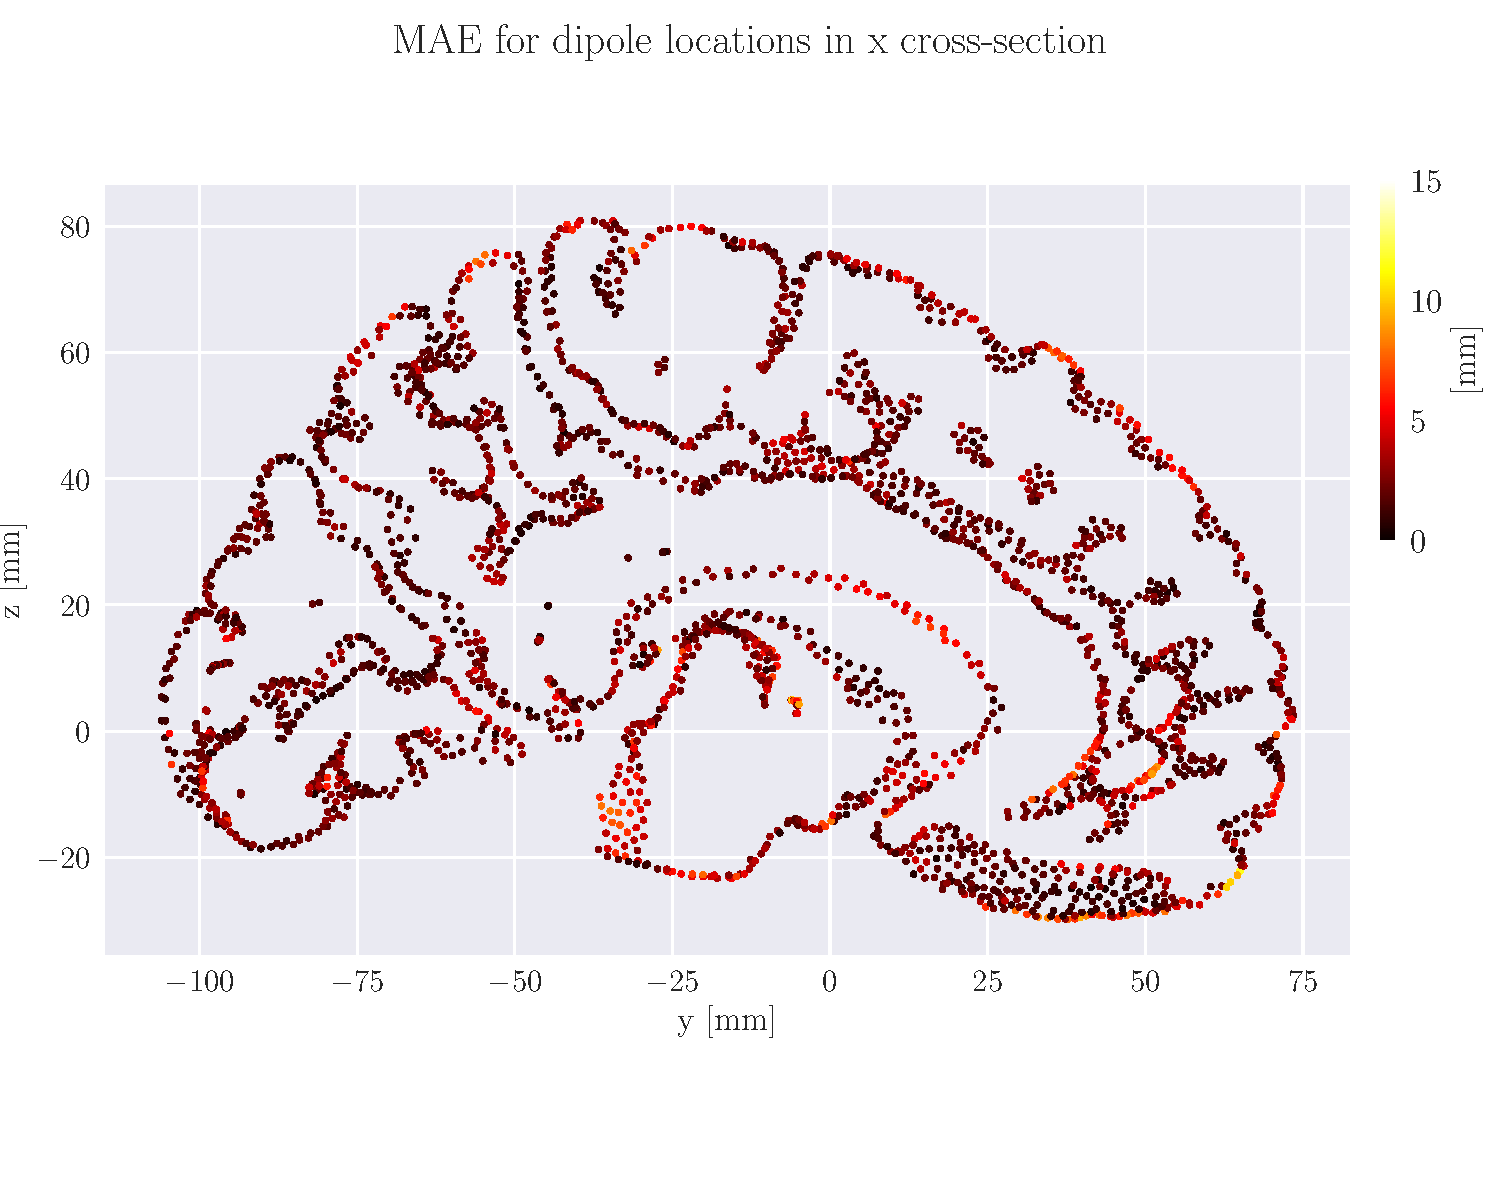
\includegraphics[width=0.7\linewidth]{figures/NEW_simple_dipole_error_Euclidean Distance_2.pdf}
    \caption{Different cross-sections of the cortex from the New York head model, seen from front, top and side. Each point represents a possible position in the cortex matrix. The color of the each point indicates the mean absolute error (MAE) of the neural network when predicting that specific dipole location.}
    \label{fig:MAE_crossections}
\end{figure}



\section{Convolution Neural Network Approach for localizing single dipole sources}

Some results for the prediction of location for single current dipoles.


\begin{figure}[!htb]
\centering
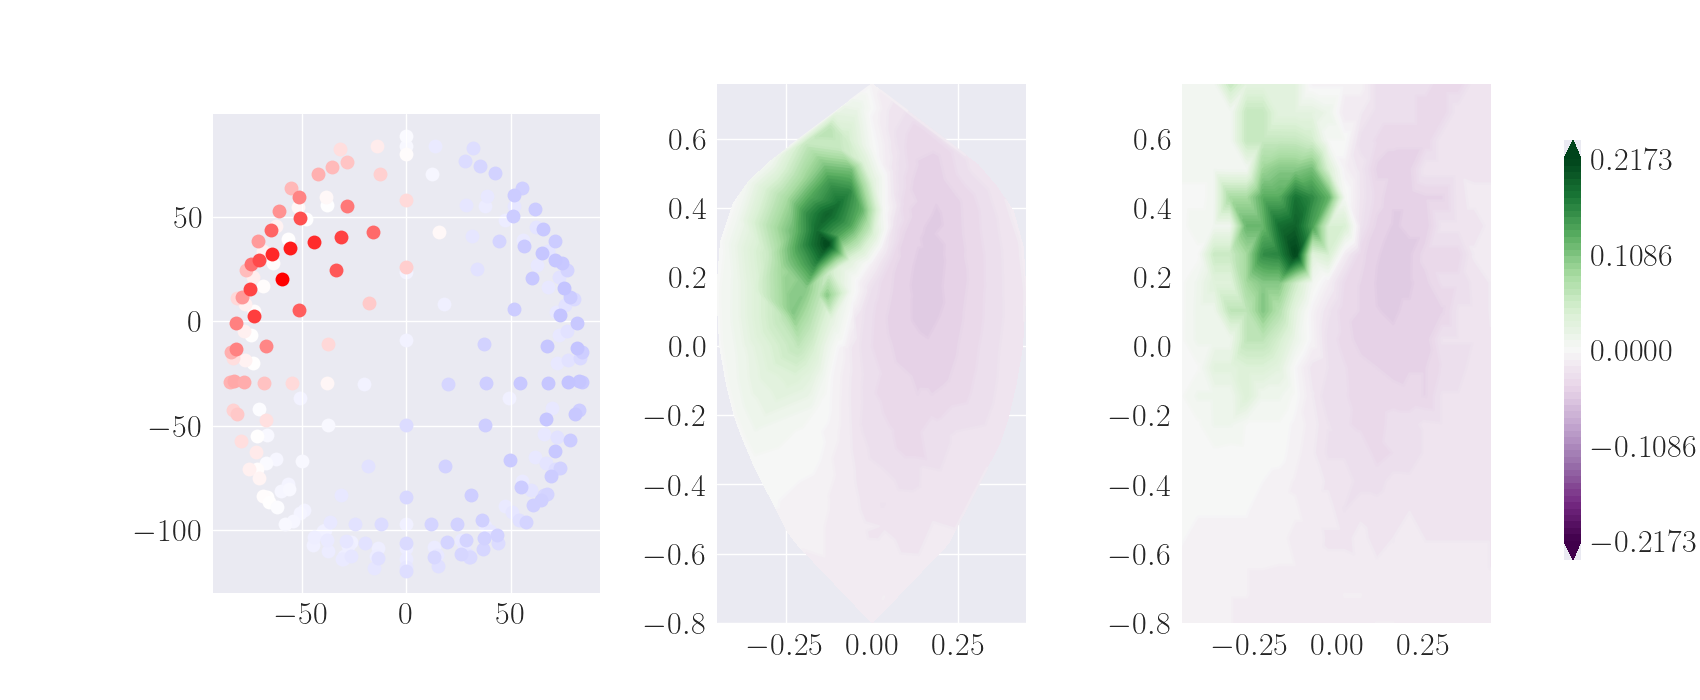
\includegraphics[width=\linewidth]{../Code/plots/finals/new_eeg_dipole_pos_0.png}
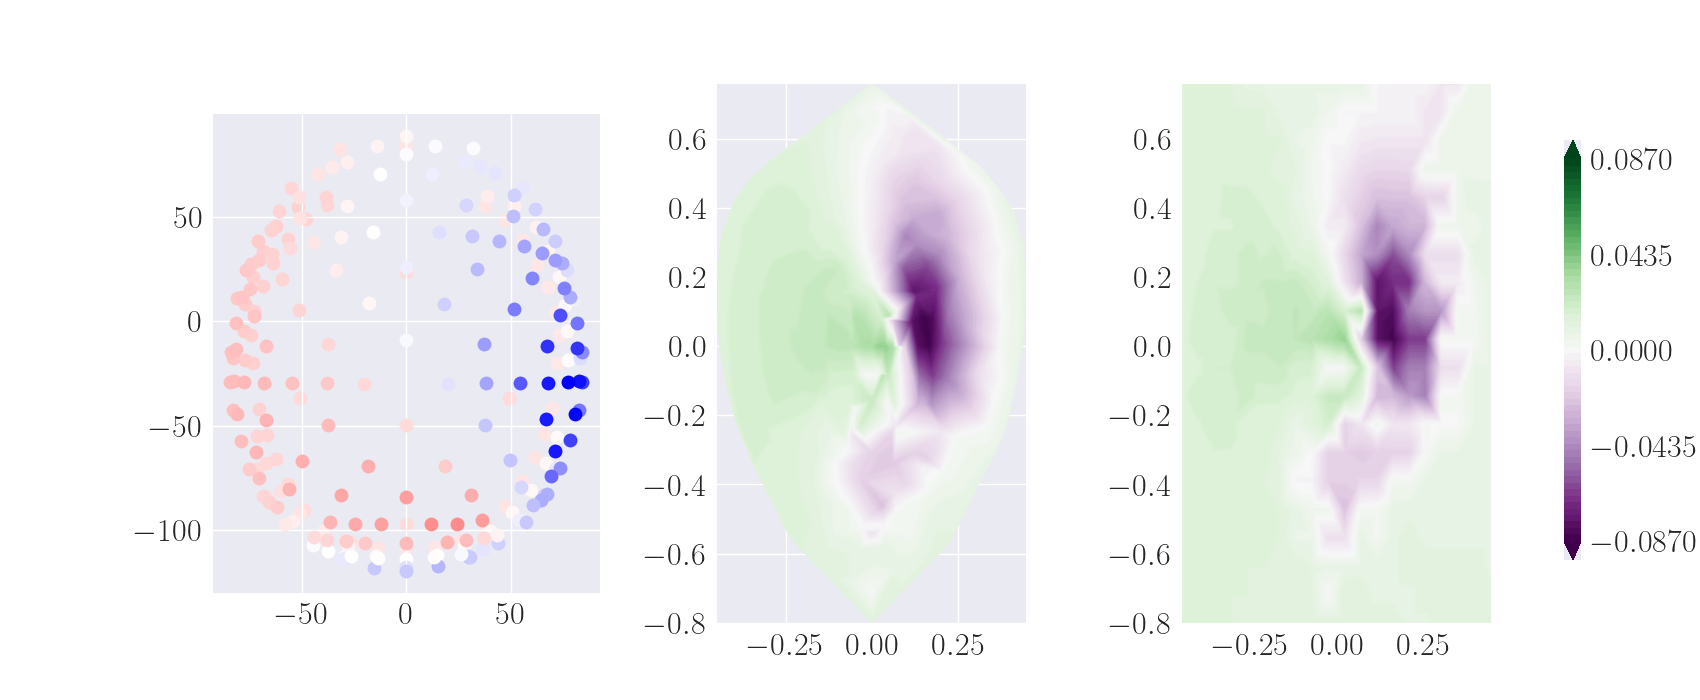
\includegraphics[width=\linewidth]{../Code/plots/finals/new_eeg_dipole_pos_4.png}
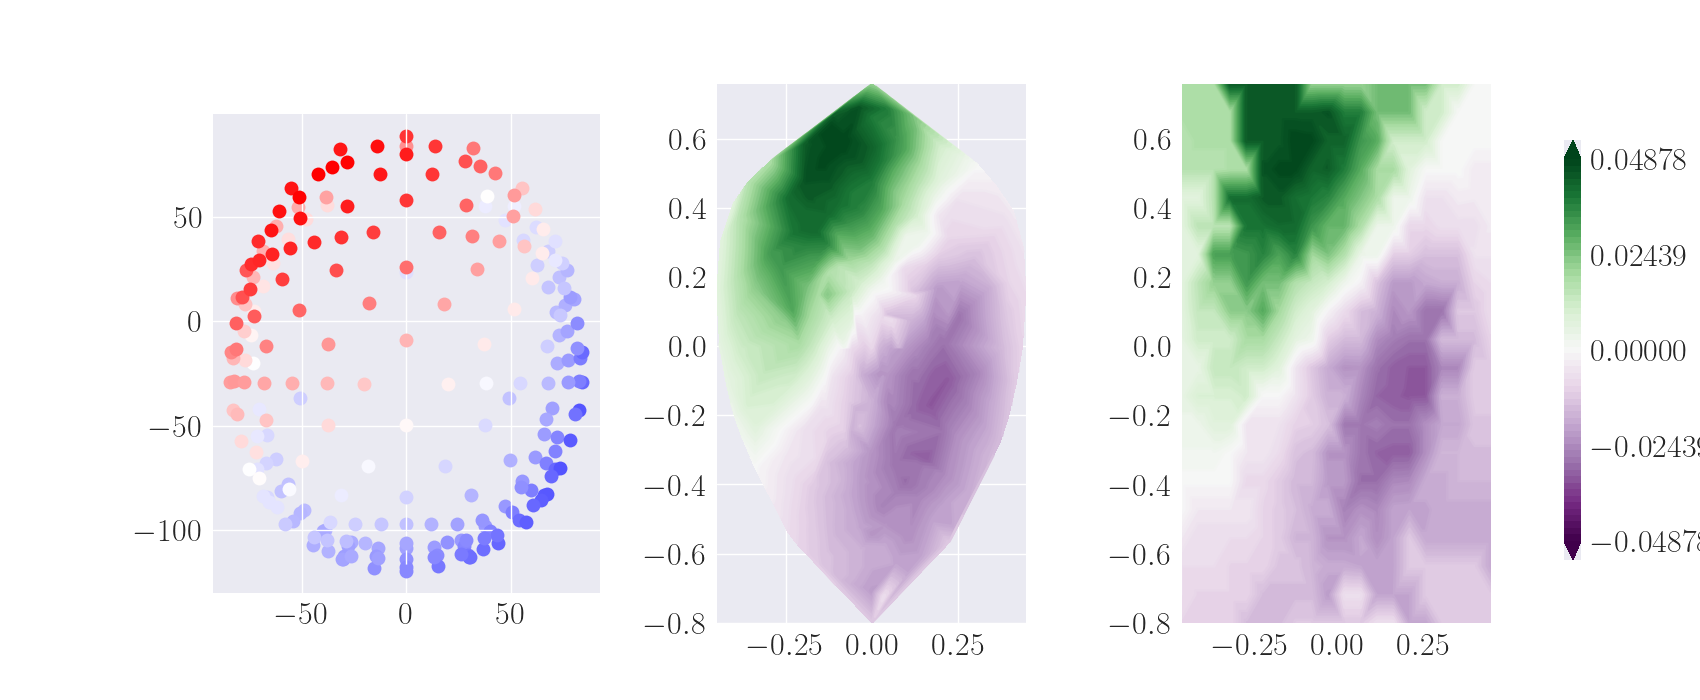
\includegraphics[width=\linewidth]{../Code/plots/finals/new_eeg_dipole_pos_6.png}

\caption{\newline
\textbf{Right}: EEG measure for 3 different samples measured in $\mu V$. \newline
\textbf{Middle and Left}: Illustration of the interpolation of the EEG data into two-dimensional matrix.}
\label{fig:eeg_dipole_pos_0}

\end{figure}

\begin{figure}[!htb]
    \centering
    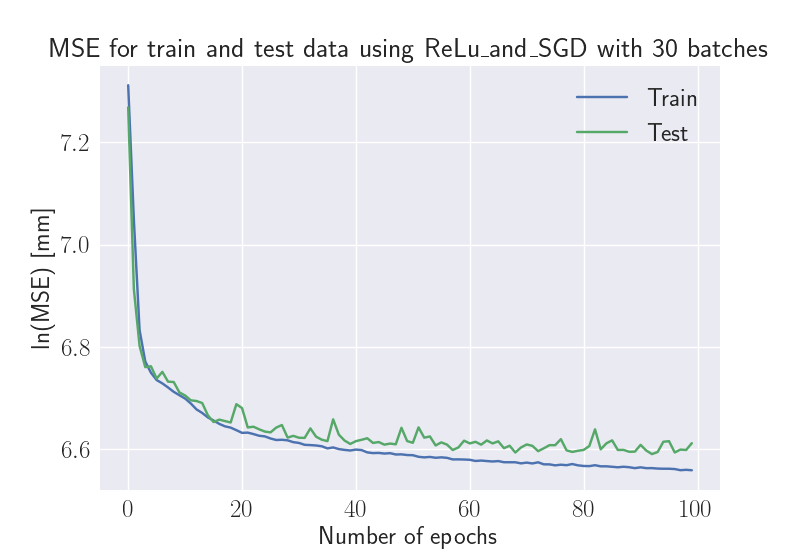
\includegraphics[width=\linewidth]{../Code/plots/finals/MSE_CNN_dipoles_2_interpolated_CNN_20x20_10000_ReLu_and_SGD_30_100.png}
    \caption{The validation accuracy for Convolutional Neural Network with 10 000 samples (20x20 matrix) with ReLU activation function. }
    \label{fig:single_dipole_accuracy_CNN_2d}
\end{figure}

% \begin{figure}[!htb]
%     \centering
%     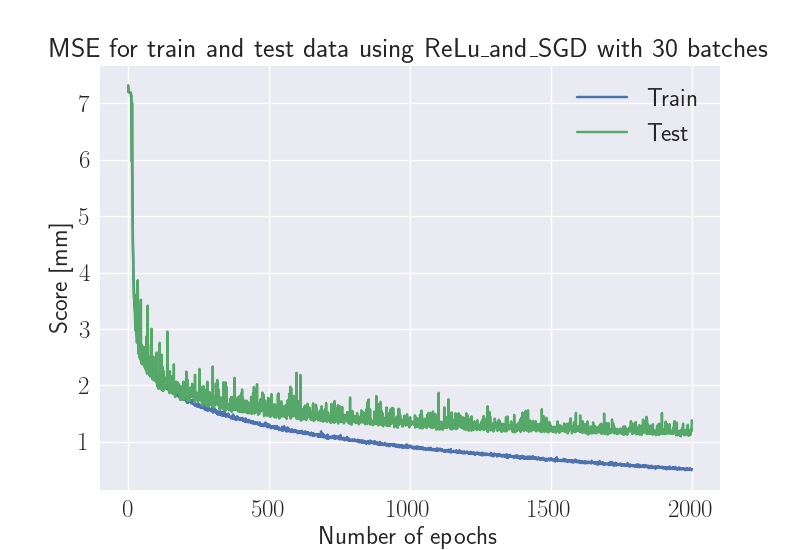
\includegraphics[width=\linewidth]{../Code/plots/CNN/MSE_interpolated_CNN_20x20_10000_ReLu_and_SGD_30_2000.png}
%     \caption{The validation accuracy for Convolutional Neural Network with 10 000 samples (20x20 interpolated matrix) with ReLU activation function. }
%     \label{fig:single_dipole_accuracy_CNN}
% \end{figure}


\end{document}
